\section{Experiments}
\label{experiments}

Our experimental evaluation of a prototype implementation of POLAR studies its general applicability and performance characteristics with a variety of benchmarks. After describing the prototype and experimental setting, we use various micro benchmarks to evaluate the behavior of different strategies and parameters and conduct end-to-end performance comparisons with DuckDB~\cite{RaasveldtM19}, Postgres~\cite{DBLP:conf/sigmod/StonebrakerR86}, and SkinnerDB~\cite{TrummerWMMJA19, TrummerWWMMJAR21} (as a representative AQP system). Our major findings are that: 
\begin{enumerate}
\item Non-invasive AQP yields robust end-to-end performance,
\item Offers substantial speedups for certain queries, especially on skewed benchmarks, and
\item Is already effective with small exploration budgets of $\leq$10\%. 
\end{enumerate}

\subsection{Experimental Setup}

\textbf{Prototype:} We implemented POLAR in DuckDB, a state-of-the-art OLAP DBMS. The prototype\footnote{On acceptance, we will share both the POLAR prototype implementation as well as scripts and artifacts of the experiments at \url{https://github.com/damslab/reproducibility}.} implementation, including several different routing and selection strategies, is ~2500 LoC and requires minimal changes to the existing DuckDB code. The input to the POLAR implementation is a query plan produced by the DuckDB optimizer, which uses equivalence sets to estimate cardinalities~\cite{thesis/Ebergen22} and the DPhyp~\cite{MoerkotteN08} algorithm to enumerate join orders.  

\textbf{Evaluation System:} We conducted all experiments on a Lenovo ThinkSystem SR635 server with a single AMD EPYC 7443P CPU at $2.85$\,GHz (24 physical/48 virtual cores), 256\,GB DDR4 RAM at 3.2\,GHz, $1\times 480\,\text{GB}$ SATA SSD, $8\times 2\,\text{TB}$ SATA HDDs (data) and Mellanox ConnectX-6 HDR/200\,Gb Infiniband. We compiled the source code with clang-12 on Ubuntu 20.04.1.

\textbf{Benchmarks:} We evaluate POLAR using the Join Order Benchmark (JOB)~\cite{JoinOrderBenchmark}, Star-Schema Benchmark (SSB)~\cite{SSB-ONeil2009-qs}, and a modified version of SSB including cross-correlation and skew (SSB-skew). We use both SSB versions with a scale factor of 10.
%
We introduce SSB-skew to evaluate how POLAR handles highly correlated and skewed data. This benchmark represents real-world data patterns and is very challenging due to cardinality estimation errors and non-uniform data clustering. SSB-skew introduces two new tables to SSB with n-to-m joins: \texttt{lineorder\_customer} and \texttt{lineorder\_part} with seasonal variance: \texttt{lineorders} may have multiple \texttt{customers} and \texttt{parts} if their order dates are within certain months each year. In other months, all \texttt{lineorders} have the same supplier. The \texttt{lineorder} table is ordered by order date. SSB-skew contains eight queries, each joining between 3 - 7 tables using a diverse set of predicates on the dimension tables.  % 
%
We considered TPC-H \cite{tpch} and JCC-H \cite{JCC-H} but did not use them because (1) their optimal join orders are well-known and often tuned for, and (2) the join orders generated by DuckDB are mostly right-deep trees which are not amenable to POLAR. We also considered the LDBC Social Network BI Workload~\cite{LDBC}, but LDBC requires advanced SQL features which are not supported by all systems we compare, and the DuckDB optimizer often generates pipelines with alternating joins and projections, which our prototype implementation does not yet support (cf. Limitations in Section~\ref{sec:limits}).
%

\subsection{Potential Benefit Analysis}
\label{sec:potential-analysis}

In a first series of experiments, we aim to understand the potential of POLAR pipelines by estimating the possible reduction in the number of intermediate tuples with optimal routing strategies. These results serve as a baseline---in terms of an upper bound---for later experiments evaluating the quality of POLAR routing strategies. Furthermore, we also examine the time per benchmark spent in amenable pipelines. Combining these measures allows estimating the ideal overall performance impact.

\textbf{Potential Reduction of Intermediates:} Table~\ref{tab:1_2_potential_savings} shows the potential performance improvements achievable with adaptive join order switching. We calculated the potential improvement by measuring the number of intermediate results for all amenable pipelines using DuckDB's default join order, the best static join order for each pipeline, and an estimated optimal routing strategy. We determined this optimal value using a multiplexer debugging mode, routing each input chunk to every legal join order and measuring the minimal number of intermediates.
%
Table~\ref{tab:1_2_potential_savings} shows that dynamic tuple routing strategies reduce the number of intermediates for all benchmarks but that the potential improvement over an ideal static join order is most significant with skewed datasets. For JOB, the best static join order produces 25.84\,M tuples compared to 107.49\,M tuples from DuckDB's default join order. Dynamic routing further improves this number to 16.92\,M tuples. This result shows that a better static join order could improve JOB to a large extent without dynamic join order switching at runtime. For SSB, neither join order switching nor better join orders considerably improve the number of intermediates. The best static join order produces 57.83\,M tuples, a moderate improvement over the 86.65\,M tuples in the default DuckDB plan, and dynamic routing makes only a slight additional improvement to 55.06\,M tuples. DuckDB's near-optimal plan for SSB is expected because the benchmark contains well-behaved FK/PK joins and uniform, non-skewed data. For SSB-skew, however, which lacks such schema information and uniform data, the potential for improvement is much higher. The default DuckDB join order produces 929.87\,M tuples, while the best static join order produces 688.90\,M tuples. Tuple routing improves this by more than an order of magnitude to 25.15\,M tuples. The routing performs so much better because no single join order can adapt to the changing data distributions while processing the clustered data. 

\begin{table}[!t]
	\centering 
	\caption{Intermediate Tuple Reduction and Coverage of Amenable Piplines -- Total number of intermediate tuples and fraction of total execution time spent in amenable pipelines.}
	\vspace{-0.3cm} \setlength\tabcolsep{5pt}
	\begin{tabular}{lrrrr}
		\toprule
		\textbf{Benchmark} & \textbf{DuckDB} & \textbf{Routing} & \textbf{Static} & \textbf{Coverage}\\
		\midrule
		JOB &     107.49 M &      16.92 M &      25.84 M & 37 \%\\
		SSB &      86.65 M &      55.06 M &      57.83 M & 68 \%\\
		SSB-skew &     929.87 M &      25.15 M &     688.90 M & 97 \%\\
		\bottomrule
	\end{tabular}
	\label{tab:1_2_potential_savings}
\end{table}


\textbf{Coverage of Amenable Pipelines:} Given DuckDB's default query plans, we measure each benchmark's total execution time and the time spent processing POLAR-amenable pipelines (\ie pipelines containing left-deep trees of two or more joins). Comparing the difference of these values yields the \textit{Coverage}, that is, the fraction of time spent in improvable pipelines. Note that the coverage also includes other operators from these pipelines, such as scans and aggregations, which POLAR cannot improve. The Coverage column in Table \ref{tab:1_2_potential_savings} shows that for JOB, DuckDB only spends 37\% of the processing time in POLAR-applicable pipelines. Consequently, almost two-thirds of the total execution time cannot be improved by POLAR. For SSB, DuckDB spends 68\% of the time in applicable pipelines, but many of them are dominated by large table scans, and the joins only account for a small portion of the time. For SSB-skew, DuckDB spends almost all of the execution time (97\%) in applicable pipelines and joins account for a large fraction of that time, providing substantial room for performance improvements.

\begin{figure}[!t]
    \centering
		\vspace{-0.1cm}
    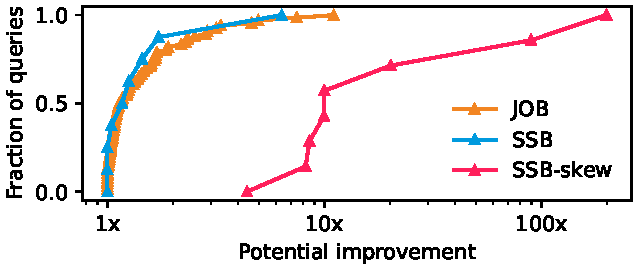
\includegraphics[width=\linewidth]{figures/1_3_potential_query_improvements.pdf}
    \vspace{-0.75cm}
		\caption{Potential Query Performance Improvement -- Estimated best case POLAR performance improvements.}
    \label{fig:1_3_potential_query_improvements}
		\vspace{-0.25cm}
\end{figure}

\textbf{Potential Query Performance Improvement:} Furthermore, we aim to assess how much the runtime of individual queries could be improved. We estimate these improvements per query by multiplying the optimal number of intermediates with the coverage of amenable pipelines (assuming a linear relationship between tuple count reduction and execution time). Figure \ref{fig:1_3_potential_query_improvements} shows a cumulative distribution function over the potential performance improvements for all queries. Some queries in both JOB and SSB can be improved by up to an order of magnitude. Queries in SSB-skew show a much larger potential for improvement: more than 50\% of queries can be improved by over an order of magnitude and some by up to 200x. 

\subsection{Micro Benchmarks}

\begin{figure*}[!t]
    \centering
    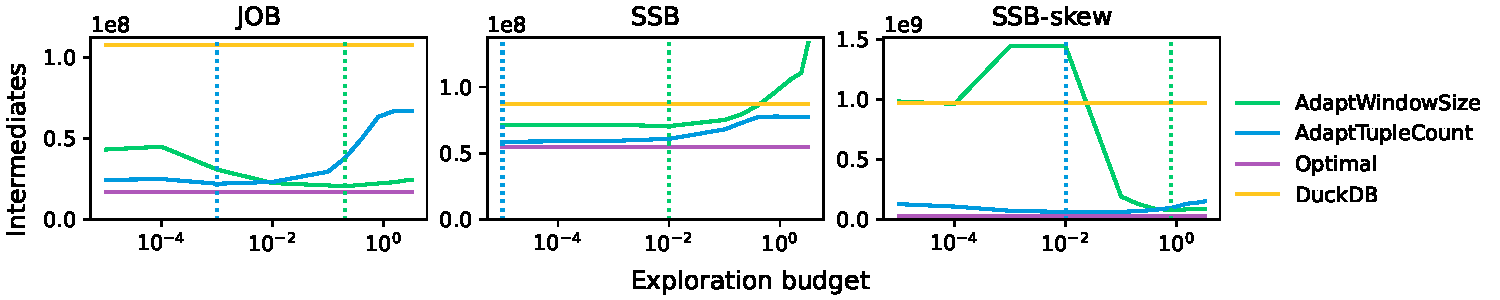
\includegraphics[width=\textwidth]{figures/2_3_routing_adaptive.pdf}
		\vspace{-0.75cm}
    \caption{Exploration Budgets -- Number of intermediate tuples for different exploration budgets. The dotted lines denote sweet spots in which the strategy generates minimal intermediates.}
    \label{fig:2_3_routing_adaptive}
\end{figure*}

To understand the trade-offs of different join selection and routing strategies, in a second series of experiments, we conduct several micro benchmarks regarding plan quality, compilation time, adaptivity, and runtime overhead. We also investigate the impact of the exploration budget on adaptivity and overhead. All micro benchmarks were executed single-threaded to isolate the effects.

\begin{table}[!t]
  \centering
  \caption{Join Order Selection -- Total number of intermediates for POLAR pipelines with different selection strategies.}
  \vspace{-0.3cm}  \setlength\tabcolsep{3.5pt}
  \begin{tabular}{lrrrr}
    \toprule
    \textbf{Enumeration} & \textbf{JOB} & \textbf{SSB} & \textbf{SSB-skew} & \textbf{JOB-ldt}\\
    \midrule
    DuckDB* &     107.49 M &      87.36 M &     967.78 M &     248.30 M\\
    Optimal &      16.92 M &      55.06 M &      25.15 M & N/A\\
    \midrule
    \textsc{GetRandom} &      16.92 M &      55.06 M &      25.15 M &     156.64 M\\
    \textsc{GetMinCard} &      16.92 M &      55.06 M &      25.15 M &     189.47 M\\
    \textsc{GetMinCardUc} &      16.92 M &      55.06 M &      25.15 M &     189.44 M\\
    \textsc{PushDown} &      17.04 M &      59.78 M &      41.46 M &     208.83 M\\
    \textsc{PullUp} &      17.22 M &      59.88 M &      53.08 M &     210.73 M\\
    \bottomrule
  \end{tabular}
  \label{tab:1_1_sel_intms}
\end{table}


\begin{figure}[!t]
    \centering \vspace{-0.1cm}
    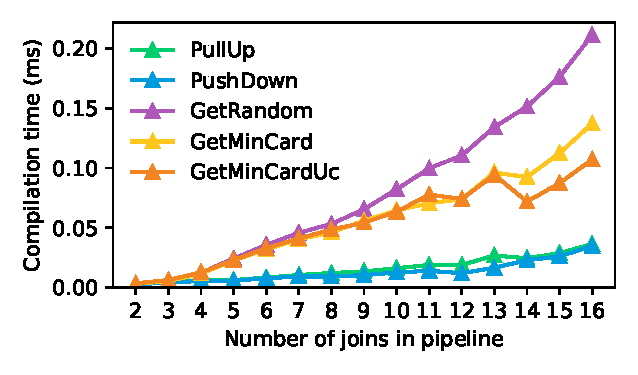
\includegraphics[width=\linewidth]{figures/2_2_enumeration_timings.pdf}
		\vspace{-0.75cm}
    \caption{Pipeline Compilation Time -- compilation time for join order selection strategies [milliseconds].}
    \label{fig:2_2_enumeration_timings}
		\vspace{-0.25cm}
\end{figure} 

\textbf{Join Order Selection:} We compare the quality of the join order selection strategies introduced in Section~\ref{sec:paths} by comparing the actual number of intermediates to the optimal number, as described in Section~\ref{sec:potential-analysis}. Table~\ref{tab:1_1_sel_intms} summarizes our findings. Since JOB, SSB, and SSB-skew only contain join pipelines with up to five relations, we can generate all possible join orders for these pipelines (cf. Section~\ref{sec:paths}). In order to stress test the different join order selection strategies, we also compared \textit{JOB-ldt}, which compiles the JOB queries using a greedy algorithm that only generates left-deep trees. For JOB and SSB, even simple strategies such as \textsc{PushDown} yield competitive results. However, for SSB-skew, the \textsc{GetRandom}, \textsc{GetMinCard}, and \textsc{GetMinCardUc} strategies produce substantially better join orders than the Default DuckDB plan because they are guaranteed to contain the optimal join order because they generate all possible candidates. For JOB-ldt, we observe that pure left-deep trees produce very large intermediates (273x larger) than a mix of bushy, left-deep, and right-deep trees. Interestingly, all join order selection strategies reduce the number of intermediates significantly (by more than 100x) but remain non-competitive compared to POLAR on top of DuckDB's default query optimizer.

\textbf{Pipeline Compilation Time:} The time required to compile a POLAR pipeline is dominated by the join order selection. We measured this compilation time for the join order selection strategies using pipelines with varying numbers of joins from JOB-ldt. Figure~\ref{fig:2_2_enumeration_timings} shows that the compilation time for \textsc{PushDown} and \textsc{PullUp} grows linearly with increasing number of relations, whereas the time of \textsc{GetRandom}, \textsc{GetMinCard}, and \textsc{GetMinCardUc} grows super-linearly. However, the absolute time required for any strategy---even for 16 joins---was less than one millisecond. Therefore, we conclude that the compilation time of POLAR pipelines is negligible compared to overall query processing times.

\textbf{Exploration Budgets:} For adaptive routing strategies, such as \textsc{AdaptTupleCount} and \textsc{AdaptWindowSize}, the quality of routing depends on the exploration budget. A higher budget allows the strategies to adapt better to path changes but also incurs larger overheads. To understand how the exploration budget affects the different workload characteristics, we execute JOB, SSB, and SSB-skew with exploration budgets from 0.001\% to 320\%. Figure \ref{fig:2_3_routing_adaptive} shows how the number of intermediates produced by the two adaptive routing strategies varies with increasing exploration budget. Both \textsc{AdaptTupleCount} and \textsc{AdaptWindowSize} achieve close to the optimal numbers of intermediates. However, the ideal exploration budgets differ for each benchmark. We attribute this effect to the differences in exploration potential, already observed in \ref{sec:potential-analysis}. While a larger budget only creates exploration overhead for SSB, such a budget is crucial to explore better join order alternatives for SSB-skew as the data distribution changes during query execution. \textsc{AdaptWindowSize} is especially sensitive to the exploration budget while \textsc{AdaptTupleCount} shows more robust behavior. Often, small exploration budgets of up to 10\% are sufficient to obtain robust performance characteristics. Moreover, the sweet spots for \textsc{AdaptWindowSize} are generally higher than for \textsc{AdaptTupleCount} as the latter consistently keeps exploring alternative join orders even under small exploration budgets.

\begin{table}[!t]
	\centering
	\caption{Intermediate Results -- Total number of intermediates per routing strategy using tuned exploration budgets.}
	\vspace{-0.3cm} \setlength\tabcolsep{7.9pt}
  \begin{tabular}{lrrr}
	\toprule
		\textbf{Routing Strategy} & \textbf{JOB} & \textbf{SSB} & \textbf{SSB-skew}\\
		\midrule
		DuckDB &     107.49 M &      86.65 M &     929.87 M\\
		Optimal &      17.01 M &      55.06 M &      25.15 M\\
        \midrule
		\textsc{InitOnce} &      43.27 M &      67.84 M &     985.83 M\\
		\textsc{Opportunistic} &      24.48 M &      58.71 M &     655.38 M\\
		\textsc{AdaptTupleCount} &      22.05 M &      \textbf{58.70 M} &      \textbf{62.93 M}\\
		\textsc{AdaptWindowSize} &      \textbf{20.51 M} &      70.53 M &     77.92 M\\
		\textsc{Backpressure} &      41.94 M &     227.33 M &     651.14 M\\
		\bottomrule
	\end{tabular}
	\label{tab:2_4_routing_all}
\end{table}


\textbf{Routing Strategies -- Intermediates:} We compare all routing strategies from Section~\ref{sec:routing_strategies} by the number of intermediate results they produce. For \textsc{AdaptTupleCount} and \textsc{AdaptWindowSize}, we set the exploration budgets according to the sweet spots found in the previous section. Table~\ref{tab:2_4_routing_all} shows that \textsc{AdaptTupleCount} performs robustly for JOB, SSB, and SSB-skew, whereas \textsc{AdaptWindowSize} produces the fewest intermediate results for JOB. \textsc{InitOnce} performs substantially worse than the adaptive strategies because it picks sub-optimal join orders whenever the initialization phase is not representative for the remaining data batches. This observation is especially pronounced for SSB-skew, where there are different optimal plans for different clusters of the data. \textsc{Backpressure} produces the most intermediate results because many executor threads process tuples in sub-optimal join orders.

\begin{table}[!t]
	\centering
	 \caption{Execution Time -- Total pipeline execution time per routing strategy [seconds].}
	 \vspace{-0.3cm}  \setlength\tabcolsep{11.4pt}
   \begin{tabular}{lrrr}
	  \toprule
		\textbf{Routing strategy} & \textbf{JOB} & \textbf{SSB} & \textbf{SSB-skew}\\
		\midrule
		DuckDB &      49.42 &       5.56 &      11.94\\
		\midrule
		\textsc{InitOnce} &      32.38 &       5.12 &      10.44\\
		\textsc{Opportunistic} &      31.44 &       6.78 &       9.40\\
		\textsc{AdaptTupleCount} &      31.44 &       7.46 &       6.50\\
		\textsc{AdaptWindowSize} &      31.02 &       5.21 &       5.36\\
		\textsc{Backpressure} &      68.35 &      14.26 &      20.65\\
		\bottomrule
	\end{tabular}
	\label{tab:3_1_pipeline}
\end{table}


\textbf{Routing Strategies -- Execution Time:} The performance of routing strategies does not solely depend on reducing intermediates. Another influential factor is how much adaptivity negatively affects vectorized execution. Tuple chunks produced by POLAR must contain vectors of sufficient size to amortize the per batch overheads, as explained in Section~\ref{sec:routing_strategies}. Therefore, we also examine the actual pipeline execution times for each routing strategy, as this is closely correlated to overall query execution time. Table \ref{tab:3_1_pipeline} shows the total pipeline execution time for different strategies, using the exploration budget sweet spots reported in the previous section. Since \textsc{AdaptWindowSize} trades path exploration granularity for better vectorization, the strategy performs best for exploration budgets that are below its sweet spots for minimal intermediates. Interestingly, the lowest number of intermediates does not necessarily lead to the lowest pipeline execution time. Despite creating substantially more intermediates, \textsc{InitOnce} performs competitively on JOB and outperforms the other strategies on SSB as it shows the cache-friendliest behavior. However, on SSB-skew, \textsc{AdaptWindowSize} has the lowest execution time and outperforms \textsc{InitOnce} substantially. \textsc{AdaptWindowSize} consistently performs better than \textsc{AdaptTupleCount}, despite creating more intermediates, which we attribute to \textsc{AdaptWindowSize}’s deferred cache flushing for sequences of routing decisions to the same join path. As \textsc{AdaptWindowSize} only performs slightly worse than \textsc{InitOnce} on SSB, we consider it to be the most robust routing strategy for the spectrum of workloads, achieving a good balance of reducing the number of intermediates and caching-friendly execution.

\begin{figure*}[!t]
    \centering
    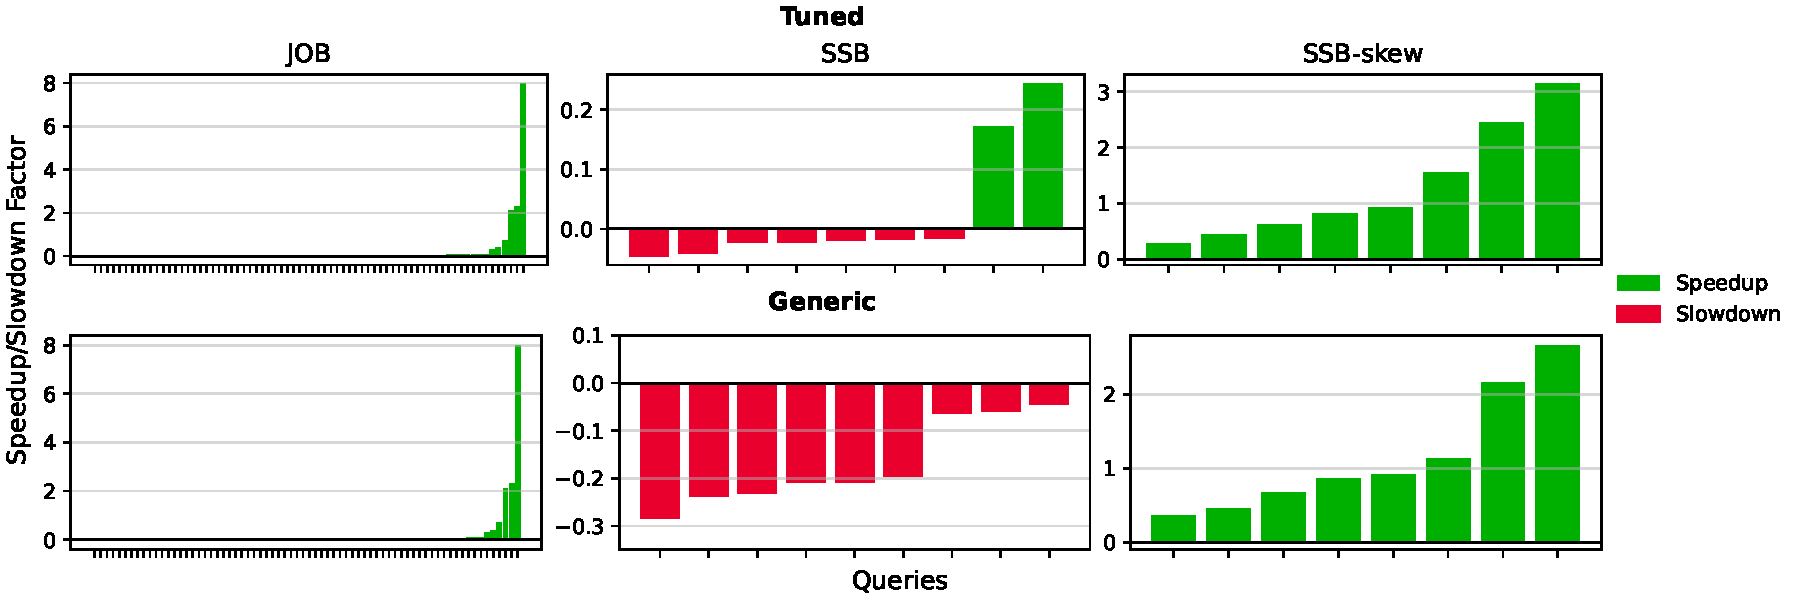
\includegraphics[width=\textwidth]{figures/3_2_rel_gains.pdf}
    \vspace{-0.55cm}
    \caption{Individual Query Performance Impact -- Query performance changes between unmodified DuckDB and POLAR. A value of +1 indicates the query was 100 \% faster (2x), and a value of -1 indicates a 100\% overhead (doubled execution time).}
    \label{fig:3_2_rel_gains}
\end{figure*}

\begin{table}[!t]
	\centering
	 \caption{Parameter Robustness -- Total pipeline execution time with generic vs. tuned exploration budgets [seconds].}
	 \vspace{-0.3cm}  \setlength\tabcolsep{8.7pt}
   \begin{tabular}{lrrr}
	  \toprule
		\textbf{Routing strategy} & \textbf{JOB} & \textbf{SSB} & \textbf{SSB-skew}\\
		\midrule
		DuckDB &      49.42 &       5.56 &      11.94\\
		\midrule
        \textsc{AdaptTupleCount} (0.01\%) &    32.73 &       7.60 &      6.84\\
		\textsc{AdaptTupleCount}-tuned &      31.44 &       7.46 &      6.50\\
        \midrule
		\textsc{AdaptWindowSize} (10\%) &      31.02 &       6.66 &       5.38\\
		\textsc{AdaptWindowSize}-tuned &      31.02 &       5.21 &       5.36\\
  		\bottomrule
	\end{tabular}
	\label{tab:3_3_parameter}
\end{table}


\textbf{Routing Strategies -- Parameter Robustness:} The previous experiment showed that routing strategies with tuned exploration budgets outperform static strategies for workloads on skewed, correlated data. However, it is not always possible to tune an exploration budget if the workload is unknown beforehand. For this reason, we evaluate the difference in execution times between a generic and tuned budget, summarized in Table~\ref{tab:3_3_parameter}. We compare the \textsc{AdaptTupleCount} and \textsc{AdaptWindowSize} routing strategies using their individual sweet spots to a static exploration budget that showed the best overall performance for JOB, SSB, and SSB-skew (0.01\% for \textsc{AdaptTupleCount}, 10\% for \textsc{AdaptWindowSize}). We observe that a generic exploration budget minimally increases execution times for \textsc{AdaptTupleCount} as this strategy generally has a robust performance for small budgets. In contrast, for \textsc{AdaptWindowSize}, a generic budget shows a larger deviation from its sweet spot for SSB but still performs better overall. Thus, we conclude that \textsc{AdaptWindowSize} is the preferable routing strategy despite its higher exploration budget sensitivity.

\subsection{End-to-End Performance Comparison}

Using the results from our micro benchmarks, we evaluate POLAR's end-to-end benchmark performance using \textsc{GetMinCard} join order selection, \textsc{AdaptWindowSize} routing strategy and both a generic 10\% exploration budget for all benchmarks (\textit{POLAR-G}), as well as tuned exploration budgets specific to each benchmark~(\mbox{\textit{POLAR-T}}), namely 10\% [JOB], 0.1\% [SSB], and 20\% [SSB-skew]. In this context, we compare POLAR with DuckDB~\cite{RaasveldtM19}, Postgres~\cite{DBLP:conf/sigmod/StonebrakerR86}, and SkinnerDB~\cite{TrummerWMMJA19}, a state-of-the-art AQP system, in both single- and multi-threaded configurations.

\begin{table}
	\centering
	\caption{Overall Performance Impact -- Single-threaded total execution time, and max execution time per query [seconds].}
		\vspace{-0.3cm} \setlength\tabcolsep{3.7pt}
   \begin{tabular}{lcccccc}
	  \toprule
		& \multicolumn{3}{c}{\textbf{Total Execution Time}} & \multicolumn{3}{c}{\textbf{Max. Query Time}}\\
         & JOB & SSB & SSB-skew & JOB & SSB & SSB-skew\\
		\midrule
		DuckDB & 135.5 & 7.8 & 12.2 & 10.7 & 1.1 & 3.6\\
        POLAR-G & 117.7 & 8.9 & 5.6 & 3.9 & 1.4 & 1.7\\
        POLAR-T & \textbf{117.7} & \textbf{7.5} & \textbf{5.6} & \textbf{3.9} & \textbf{0.9} & \textbf{1.7} \\
        Speedup & 1.15x & 1.04x & \textbf{\color{red}2.18x} & \textbf{\color{red}2.74x} & 1.22x & \textbf{\color{red}2.12x}\\
		\bottomrule
	\end{tabular}
	\label{tab:3_4_endtoend}
\end{table}


\begin{figure*}
    \centering
    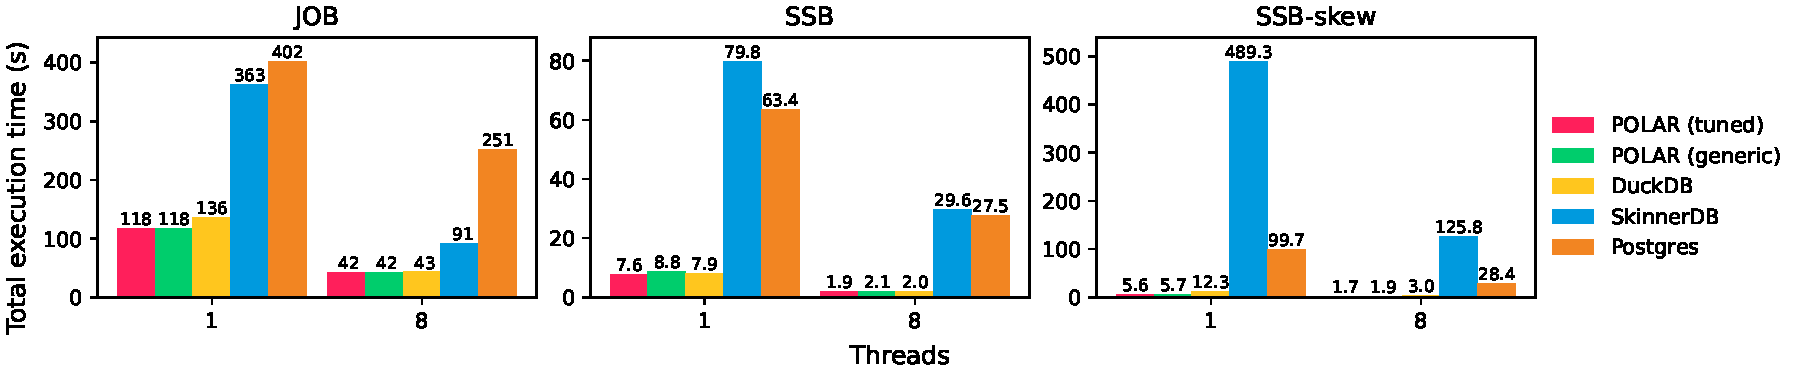
\includegraphics[width=\textwidth]{figures/4_1_total.pdf}
    \vspace{-0.55cm}
    \caption{AQP System Comparison -- Total execution times for JOB, SSB, and SSB-skew, using 1 and 8 threads [seconds].}
    \label{fig:4_1_total}
\end{figure*}

\textbf{Overall Performance Impact:} Table~\ref{tab:3_4_endtoend} shows the total end-to-end, single-threaded execution time---as well as the maximum query execution times---for DuckDB, POLAR-G, and POLAR-T on the different benchmarks. POLAR-T provides moderate total end-to-end performance improvements of 1.15x and 1.04x for JOB and SSB, respectively, and a substantial 2.18x end-to-end improvement for SSB-skew. Additionally, POLAR-T significantly improves the worst-performing queries by 2.74x in JOB, and 2.12x in SSB-skew. POLAR-G performs as well as POLAR-T for JOB and SSB-skew but shows more overhead on SSB. Generally, POLAR improves robustness by ensuring good execution time for all queries, even those where we would otherwise pick bad plans. 

\textbf{Individual Query Performance Impact:} Figure~\ref{fig:3_2_rel_gains} displays speedups and slowdowns for each query with POLAR-amenable pipelines in JOB, SSB, and SSB-skew. A value of 1 indicates an improvement of 100\% (\ie half the execution time or 2x), whereas a value of -1 indicates double the execution time. For most JOB queries, POLAR has no positive or negative effect on the execution time. However, for a few queries, POLAR substantially reduces the execution time by up to 9x. The two queries with the largest speedups are also the longest-running queries in the benchmark. On SSB, the POLAR overhead increases the execution time for most queries, as expected, given how close to optimal the original join plans are. POLAR's overhead is smaller than 5\% for any query when the exploration budget is properly tuned. With the generic configuration, POLAR's overhead is up to 28\%. Finally, all queries in SSB-skew improve with POLAR, up to 4x in some cases. Therefore, POLAR-T achieves substantial performance and robustness improvements with negligible overhead. With a generic budget, queries on uniform data may incur a perceivable overhead due to plan exploration and impact on vectorization at runtime. However, this moderate overhead is an acceptable price to pay for increased robustness, and the overhead could be further decreased when specializing POLAR to the underlying runtime characteristics.

\textbf{AQP System Comparison:} To contextualize POLAR's performance, we compare POLAR, DuckDB, Postgres, and SkinnerDB, measuring the total execution time in single- and multi-threaded (8 threads) configurations. We allow SkinnerDB to cache indexes on all join columns in memory to reduce its pre-processing time. We use Postgres 12.15 and set \texttt{max\_parallel\_workers\_per\_gather} to control the level of parallelism. Moreover, we disable nested-loop joins to prevent Postgres from choosing aggressive plans with fatal performance. Figure~\ref{fig:4_1_total} shows that with a tuned exploration budget, POLAR performs equally or better than DuckDB, SkinnerDB, and Postgres on all benchmarks and configurations. Using a generic exploration budget, POLAR performs slightly worse but still outperforms the other systems on JOB and SSB-skew. On SSB, the generic POLAR configuration performs worse than DuckDB for single-threaded but is comparable (2.1 vs 2.0 seconds) for multi-threaded execution. The increased parallelism seems to hide performance penalties from reduced vectorization opportunities. On SSB-skew, POLAR with both tuned and generic exploration budgets outperforms DuckDB by more than 2x single-threaded and more than 1.5x multi-threaded. SkinnerDB and Postgres both show much higher total execution times than POLAR and DuckDB, as expected, given their different target workloads and runtime systems. SkinnerDB performs worst on SSB and SSB-skew. On SSB (single- and multi-threaded) and SSB-skew (single-threaded), POLAR roughly outperforms SkinnerDB by 10x, whereas on multi-threaded SSB-skew, POLAR exhibits an improvement of 66-74x. We attribute this difference to the fact that SkinnerDB is restricted to choosing a single left-deep join plan and its non-vectorized execution. For SSB-skew, the uneven data distribution means any single join order, even if robust, can not capture the changing data skew over the course of the query's execution. Our performance experiments demonstrate the benefits of a non-invasive, bounded-overhead system design in an engine designed for analytic workloads. In contrast to invasive AQP systems, POLAR favors reusing existing database components and original plans resulting in competitive performance and much greater robustness with modest overhead.
